\documentclass[1p]{elsarticle_modified}
%\bibliographystyle{elsarticle-num}

%\usepackage[colorlinks]{hyperref}
%\usepackage{abbrmath_seonhwa} %\Abb, \Ascr, \Acal ,\Abf, \Afrak
\usepackage{amsfonts}
\usepackage{amssymb}
\usepackage{amsmath}
\usepackage{amsthm}
\usepackage{scalefnt}
\usepackage{amsbsy}
\usepackage{kotex}
\usepackage{caption}
\usepackage{subfig}
\usepackage{color}
\usepackage{graphicx}
\usepackage{xcolor} %% white, black, red, green, blue, cyan, magenta, yellow
\usepackage{float}
\usepackage{setspace}
\usepackage{hyperref}

\usepackage{tikz}
\usetikzlibrary{arrows}

\usepackage{multirow}
\usepackage{array} % fixed length table
\usepackage{hhline}

%%%%%%%%%%%%%%%%%%%%%
\makeatletter
\renewcommand*\env@matrix[1][\arraystretch]{%
	\edef\arraystretch{#1}%
	\hskip -\arraycolsep
	\let\@ifnextchar\new@ifnextchar
	\array{*\c@MaxMatrixCols c}}
\makeatother %https://tex.stackexchange.com/questions/14071/how-can-i-increase-the-line-spacing-in-a-matrix
%%%%%%%%%%%%%%%

\usepackage[normalem]{ulem}

\newcommand{\msout}[1]{\ifmmode\text{\sout{\ensuremath{#1}}}\else\sout{#1}\fi}
%SOURCE: \msout is \stkout macro in https://tex.stackexchange.com/questions/20609/strikeout-in-math-mode

\newcommand{\cancel}[1]{
	\ifmmode
	{\color{red}\msout{#1}}
	\else
	{\color{red}\sout{#1}}
	\fi
}

\newcommand{\add}[1]{
	{\color{blue}\uwave{#1}}
}

\newcommand{\replace}[2]{
	\ifmmode
	{\color{red}\msout{#1}}{\color{blue}\uwave{#2}}
	\else
	{\color{red}\sout{#1}}{\color{blue}\uwave{#2}}
	\fi
}

\newcommand{\Sol}{\mathcal{S}} %segment
\newcommand{\D}{D} %diagram
\newcommand{\A}{\mathcal{A}} %arc


%%%%%%%%%%%%%%%%%%%%%%%%%%%%%5 test

\def\sl{\operatorname{\textup{SL}}(2,\Cbb)}
\def\psl{\operatorname{\textup{PSL}}(2,\Cbb)}
\def\quan{\mkern 1mu \triangleright \mkern 1mu}

\theoremstyle{definition}
\newtheorem{thm}{Theorem}[section]
\newtheorem{prop}[thm]{Proposition}
\newtheorem{lem}[thm]{Lemma}
\newtheorem{ques}[thm]{Question}
\newtheorem{cor}[thm]{Corollary}
\newtheorem{defn}[thm]{Definition}
\newtheorem{exam}[thm]{Example}
\newtheorem{rmk}[thm]{Remark}
\newtheorem{alg}[thm]{Algorithm}

\newcommand{\I}{\sqrt{-1}}
\begin{document}

%\begin{frontmatter}
%
%\title{Boundary parabolic representations of knots up to 8 crossings}
%
%%% Group authors per affiliation:
%\author{Yunhi Cho} 
%\address{Department of Mathematics, University of Seoul, Seoul, Korea}
%\ead{yhcho@uos.ac.kr}
%
%
%\author{Seonhwa Kim} %\fnref{s_kim}}
%\address{Center for Geometry and Physics, Institute for Basic Science, Pohang, 37673, Korea}
%\ead{ryeona17@ibs.re.kr}
%
%\author{Hyuk Kim}
%\address{Department of Mathematical Sciences, Seoul National University, Seoul 08826, Korea}
%\ead{hyukkim@snu.ac.kr}
%
%\author{Seokbeom Yoon}
%\address{Department of Mathematical Sciences, Seoul National University, Seoul, 08826,  Korea}
%\ead{sbyoon15@snu.ac.kr}
%
%\begin{abstract}
%We find all boundary parabolic representation of knots up to 8 crossings.
%
%\end{abstract}
%\begin{keyword}
%    \MSC[2010] 57M25 
%\end{keyword}
%
%\end{frontmatter}

%\linenumbers
%\tableofcontents
%
\newcommand\colored[1]{\textcolor{white}{\rule[-0.35ex]{0.8em}{1.4ex}}\kern-0.8em\color{red} #1}%
%\newcommand\colored[1]{\textcolor{white}{ #1}\kern-2.17ex	\textcolor{white}{ #1}\kern-1.81ex	\textcolor{white}{ #1}\kern-2.15ex\color{red}#1	}

{\Large $\underline{12a_{0120}~(K12a_{0120})}$}

\setlength{\tabcolsep}{10pt}
\renewcommand{\arraystretch}{1.6}
\vspace{1cm}\begin{tabular}{m{100pt}>{\centering\arraybackslash}m{274pt}}
\multirow{5}{120pt}{
	\centering
	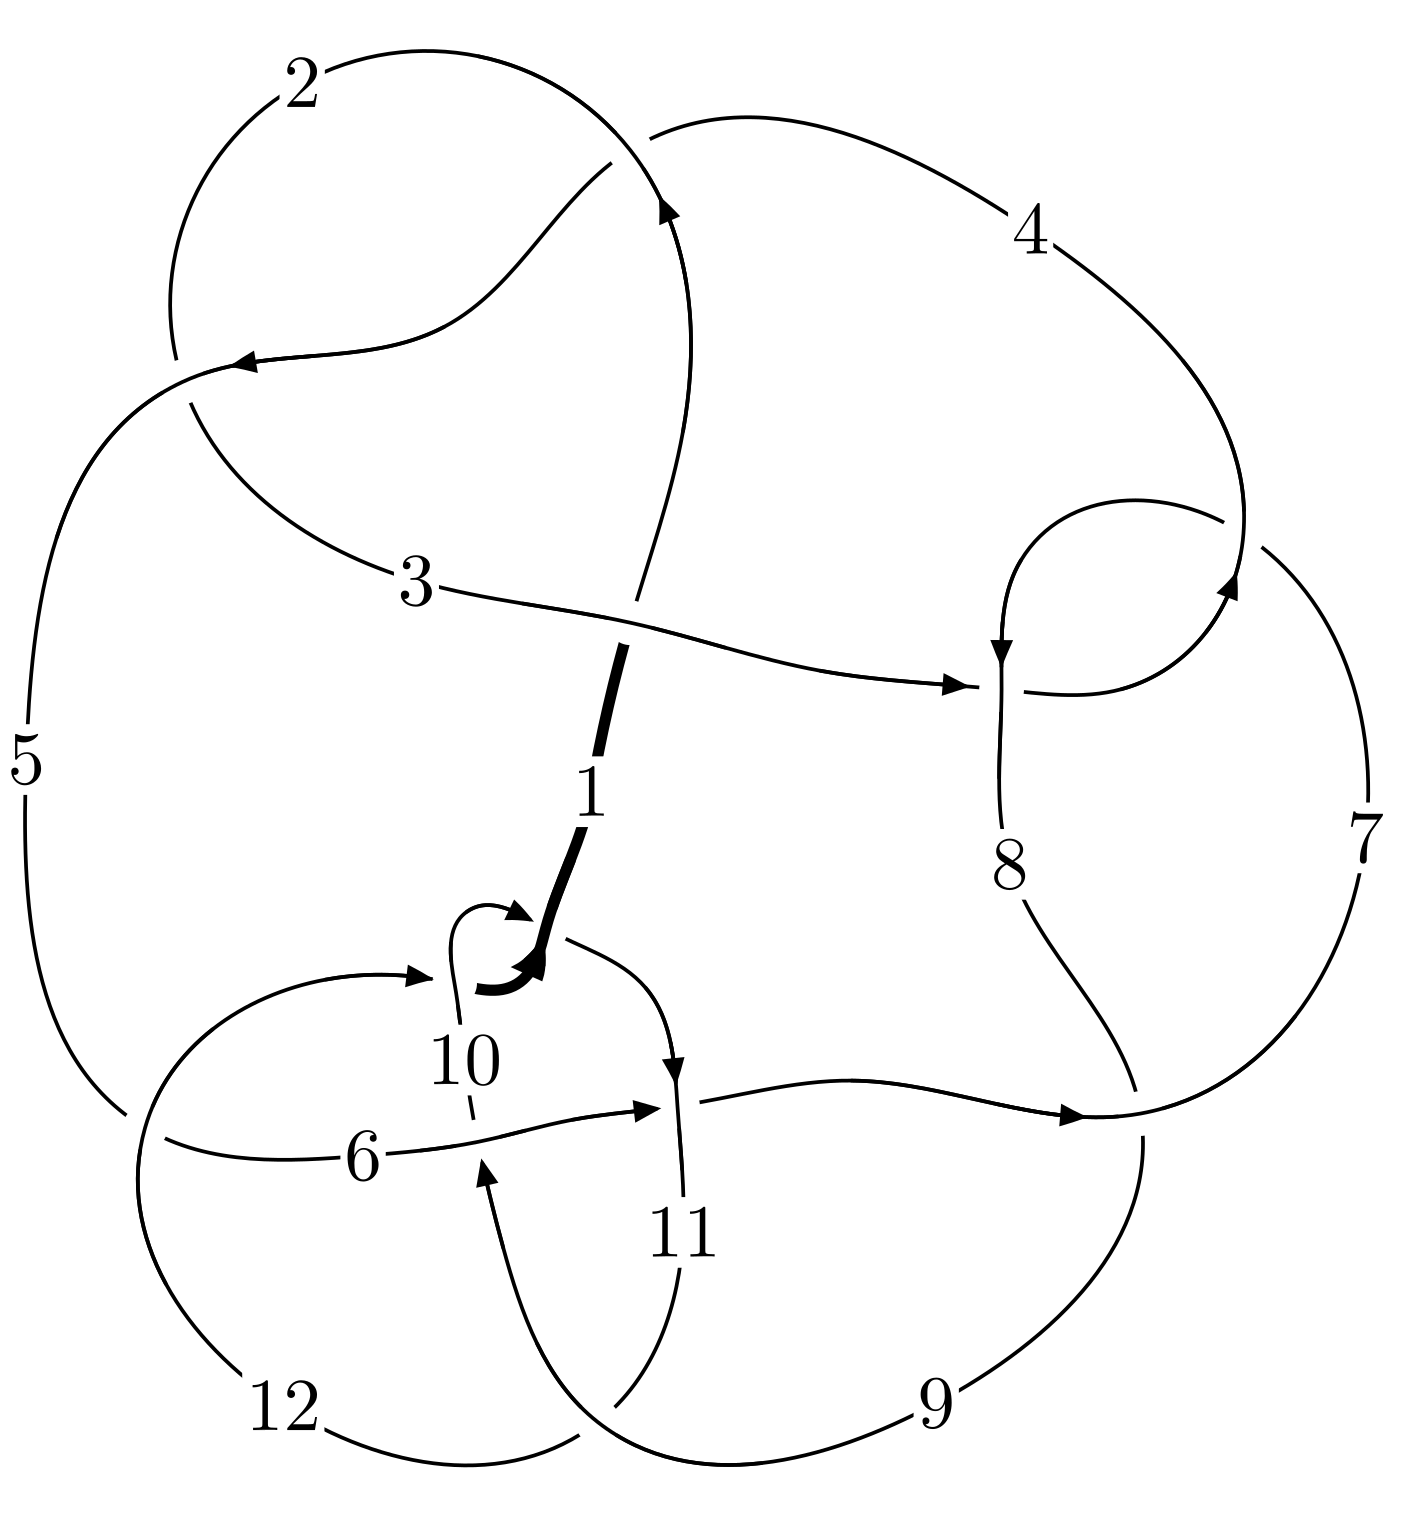
\includegraphics[width=112pt]{../../../GIT/diagram.site/Diagrams/png/921_12a_0120.png}\\
\ \ \ A knot diagram\footnotemark}&
\allowdisplaybreaks
\textbf{Linearized knot diagam} \\
\cline{2-2}
 &
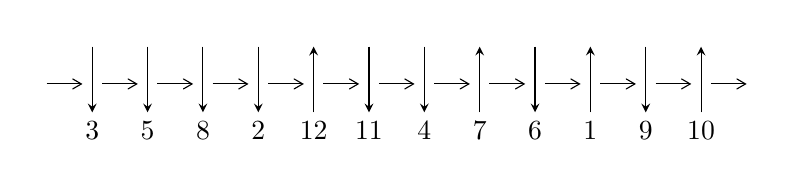
\begin{tikzpicture}[x=20pt, y=17pt]
	% nodes
	\node (C0) at (0, 0) {};
	\node (C1) at (1, 0) {};
	\node (C1U) at (1, +1) {};
	\node (C1D) at (1, -1) {3};

	\node (C2) at (2, 0) {};
	\node (C2U) at (2, +1) {};
	\node (C2D) at (2, -1) {5};

	\node (C3) at (3, 0) {};
	\node (C3U) at (3, +1) {};
	\node (C3D) at (3, -1) {8};

	\node (C4) at (4, 0) {};
	\node (C4U) at (4, +1) {};
	\node (C4D) at (4, -1) {2};

	\node (C5) at (5, 0) {};
	\node (C5U) at (5, +1) {};
	\node (C5D) at (5, -1) {12};

	\node (C6) at (6, 0) {};
	\node (C6U) at (6, +1) {};
	\node (C6D) at (6, -1) {11};

	\node (C7) at (7, 0) {};
	\node (C7U) at (7, +1) {};
	\node (C7D) at (7, -1) {4};

	\node (C8) at (8, 0) {};
	\node (C8U) at (8, +1) {};
	\node (C8D) at (8, -1) {7};

	\node (C9) at (9, 0) {};
	\node (C9U) at (9, +1) {};
	\node (C9D) at (9, -1) {6};

	\node (C10) at (10, 0) {};
	\node (C10U) at (10, +1) {};
	\node (C10D) at (10, -1) {1};

	\node (C11) at (11, 0) {};
	\node (C11U) at (11, +1) {};
	\node (C11D) at (11, -1) {9};

	\node (C12) at (12, 0) {};
	\node (C12U) at (12, +1) {};
	\node (C12D) at (12, -1) {10};
	\node (C13) at (13, 0) {};

	% arrows
	\draw[->,>={angle 60}]
	(C0) edge (C1) (C1) edge (C2) (C2) edge (C3) (C3) edge (C4) (C4) edge (C5) (C5) edge (C6) (C6) edge (C7) (C7) edge (C8) (C8) edge (C9) (C9) edge (C10) (C10) edge (C11) (C11) edge (C12) (C12) edge (C13) ;	\draw[->,>=stealth]
	(C1U) edge (C1D) (C2U) edge (C2D) (C3U) edge (C3D) (C4U) edge (C4D) (C5D) edge (C5U) (C6U) edge (C6D) (C7U) edge (C7D) (C8D) edge (C8U) (C9U) edge (C9D) (C10D) edge (C10U) (C11U) edge (C11D) (C12D) edge (C12U) ;
	\end{tikzpicture} \\
\hhline{~~} \\& 
\textbf{Solving Sequence} \\ \cline{2-2} 
 &
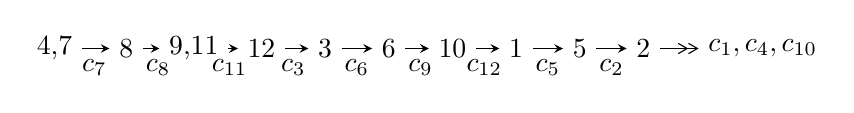
\begin{tikzpicture}[x=23pt, y=7pt]
	% node
	\node (A0) at (-1/8, 0) {4,7};
	\node (A1) at (1, 0) {8};
	\node (A2) at (33/16, 0) {9,11};
	\node (A3) at (25/8, 0) {12};
	\node (A4) at (33/8, 0) {3};
	\node (A5) at (41/8, 0) {6};
	\node (A6) at (49/8, 0) {10};
	\node (A7) at (57/8, 0) {1};
	\node (A8) at (65/8, 0) {5};
	\node (A9) at (73/8, 0) {2};
	\node (C1) at (1/2, -1) {$c_{7}$};
	\node (C2) at (3/2, -1) {$c_{8}$};
	\node (C3) at (21/8, -1) {$c_{11}$};
	\node (C4) at (29/8, -1) {$c_{3}$};
	\node (C5) at (37/8, -1) {$c_{6}$};
	\node (C6) at (45/8, -1) {$c_{9}$};
	\node (C7) at (53/8, -1) {$c_{12}$};
	\node (C8) at (61/8, -1) {$c_{5}$};
	\node (C9) at (69/8, -1) {$c_{2}$};
	\node (A10) at (11, 0) {$c_{1},c_{4},c_{10}$};

	% edge
	\draw[->,>=stealth]	
	(A0) edge (A1) (A1) edge (A2) (A2) edge (A3) (A3) edge (A4) (A4) edge (A5) (A5) edge (A6) (A6) edge (A7) (A7) edge (A8) (A8) edge (A9) ;
	\draw[->>,>={angle 60}]	
	(A9) edge (A10);
\end{tikzpicture} \\ 

\end{tabular} \\

\footnotetext{
The image of knot diagram is generated by the software ``\textbf{Draw programme}" developed by Andrew Bartholomew(\url{http://www.layer8.co.uk/maths/draw/index.htm\#Running-draw}), where we modified some parts for our purpose(\url{https://github.com/CATsTAILs/LinksPainter}).
}\phantom \\ \newline 
\centering \textbf{Ideals for irreducible components\footnotemark of $X_{\text{par}}$} 
 
\begin{align*}
I^u_{1}&=\langle 
-1.75706\times10^{313} u^{125}+2.01574\times10^{313} u^{124}+\cdots+4.16145\times10^{314} b+9.40803\times10^{315},\\
\phantom{I^u_{1}}&\phantom{= \langle  }-1.92978\times10^{314} u^{125}-2.84524\times10^{314} u^{124}+\cdots+1.66458\times10^{315} a+4.14260\times10^{316},\\
\phantom{I^u_{1}}&\phantom{= \langle  }u^{126}+2 u^{125}+\cdots+192 u+64\rangle \\
I^u_{2}&=\langle 
-2 u^2+b- u-3,\;-7 u^2+a-3 u-12,\;u^3+u^2+2 u+1\rangle \\
\\
I^v_{1}&=\langle 
a,\;-5 v^5+46 v^4-122 v^3+163 v^2+69 b+27 v+86,\;v^6-3 v^5+6 v^4+5 v^2- v+1\rangle \\
\end{align*}
\raggedright * 3 irreducible components of $\dim_{\mathbb{C}}=0$, with total 135 representations.\\
\footnotetext{All coefficients of polynomials are rational numbers. But the coefficients are sometimes approximated in decimal forms when there is not enough margin.}
\newpage
\renewcommand{\arraystretch}{1}
\centering \section*{I. $I^u_{1}= \langle -1.76\times10^{313} u^{125}+2.02\times10^{313} u^{124}+\cdots+4.16\times10^{314} b+9.41\times10^{315},\;-1.93\times10^{314} u^{125}-2.85\times10^{314} u^{124}+\cdots+1.66\times10^{315} a+4.14\times10^{316},\;u^{126}+2 u^{125}+\cdots+192 u+64 \rangle$}
\flushleft \textbf{(i) Arc colorings}\\
\begin{tabular}{m{7pt} m{180pt} m{7pt} m{180pt} }
\flushright $a_{4}=$&$\begin{pmatrix}0\\u\end{pmatrix}$ \\
\flushright $a_{7}=$&$\begin{pmatrix}1\\0\end{pmatrix}$ \\
\flushright $a_{8}=$&$\begin{pmatrix}1\\u^2\end{pmatrix}$ \\
\flushright $a_{9}=$&$\begin{pmatrix}u^2+1\\u^2\end{pmatrix}$ \\
\flushright $a_{11}=$&$\begin{pmatrix}0.115932 u^{125}+0.170928 u^{124}+\cdots-21.4968 u-24.8867\\0.0422222 u^{125}-0.0484384 u^{124}+\cdots-57.8079 u-22.6075\end{pmatrix}$ \\
\flushright $a_{12}=$&$\begin{pmatrix}0.0835374 u^{125}+0.170647 u^{124}+\cdots+7.57394 u-11.3645\\0.0603937 u^{125}-0.0175989 u^{124}+\cdots-68.0136 u-27.0882\end{pmatrix}$ \\
\flushright $a_{3}=$&$\begin{pmatrix}u\\u^3+u\end{pmatrix}$ \\
\flushright $a_{6}=$&$\begin{pmatrix}0.0131721 u^{125}+0.160291 u^{124}+\cdots+31.9622 u+2.52399\\-0.0309936 u^{125}-0.0501114 u^{124}+\cdots+21.4480 u+2.89453\end{pmatrix}$ \\
\flushright $a_{10}=$&$\begin{pmatrix}0.135778 u^{125}+0.231184 u^{124}+\cdots-24.6169 u-20.6261\\-0.0157486 u^{125}-0.0505249 u^{124}+\cdots-45.0908 u-12.3200\end{pmatrix}$ \\
\flushright $a_{1}=$&$\begin{pmatrix}0.134423 u^{125}+0.249675 u^{124}+\cdots-15.7540 u-12.1955\\-0.0161903 u^{125}-0.0611574 u^{124}+\cdots-50.9747 u-14.3007\end{pmatrix}$ \\
\flushright $a_{5}=$&$\begin{pmatrix}0.0842320 u^{125}+0.177889 u^{124}+\cdots+30.2985 u+3.33220\\-0.0501911 u^{125}-0.0717859 u^{124}+\cdots+46.0525 u+15.5277\end{pmatrix}$ \\
\flushright $a_{2}=$&$\begin{pmatrix}-0.116123 u^{125}-0.204715 u^{124}+\cdots+22.9544 u+12.7987\\0.0366348 u^{125}+0.0898334 u^{124}+\cdots+55.3988 u+14.3689\end{pmatrix}$\\&\end{tabular}
\flushleft \textbf{(ii) Obstruction class $= -1$}\\~\\
\flushleft \textbf{(iii) Cusp Shapes $= -0.597782 u^{125}-0.910341 u^{124}+\cdots-72.2510 u+19.0666$}\\~\\
\newpage\renewcommand{\arraystretch}{1}
\flushleft \textbf{(iv) u-Polynomials at the component}\newline \\
\begin{tabular}{m{50pt}|m{274pt}}
Crossings & \hspace{64pt}u-Polynomials at each crossing \\
\hline $$\begin{aligned}c_{1}\end{aligned}$$&$\begin{aligned}
&u^{126}+68 u^{125}+\cdots-17 u+1
\end{aligned}$\\
\hline $$\begin{aligned}c_{2},c_{4}\end{aligned}$$&$\begin{aligned}
&u^{126}-8 u^{125}+\cdots-9 u+1
\end{aligned}$\\
\hline $$\begin{aligned}c_{3},c_{7}\end{aligned}$$&$\begin{aligned}
&u^{126}+2 u^{125}+\cdots+192 u+64
\end{aligned}$\\
\hline $$\begin{aligned}c_{5}\end{aligned}$$&$\begin{aligned}
&u^{126}+4 u^{125}+\cdots-1174 u-44
\end{aligned}$\\
\hline $$\begin{aligned}c_{6}\end{aligned}$$&$\begin{aligned}
&u^{126}-65 u^{124}+\cdots+4405 u-191
\end{aligned}$\\
\hline $$\begin{aligned}c_{8}\end{aligned}$$&$\begin{aligned}
&u^{126}-42 u^{125}+\cdots-118784 u+4096
\end{aligned}$\\
\hline $$\begin{aligned}c_{9}\end{aligned}$$&$\begin{aligned}
&u^{126}-9 u^{125}+\cdots+2 u-1
\end{aligned}$\\
\hline $$\begin{aligned}c_{10},c_{12}\end{aligned}$$&$\begin{aligned}
&u^{126}+5 u^{125}+\cdots-43 u-1
\end{aligned}$\\
\hline $$\begin{aligned}c_{11}\end{aligned}$$&$\begin{aligned}
&u^{126}-20 u^{125}+\cdots+124 u+8
\end{aligned}$\\
\hline
\end{tabular}\\~\\
\newpage\renewcommand{\arraystretch}{1}
\flushleft \textbf{(v) Riley Polynomials at the component}\newline \\
\begin{tabular}{m{50pt}|m{274pt}}
Crossings & \hspace{64pt}Riley Polynomials at each crossing \\
\hline $$\begin{aligned}c_{1}\end{aligned}$$&$\begin{aligned}
&y^{126}-12 y^{125}+\cdots-363 y+1
\end{aligned}$\\
\hline $$\begin{aligned}c_{2},c_{4}\end{aligned}$$&$\begin{aligned}
&y^{126}-68 y^{125}+\cdots+17 y+1
\end{aligned}$\\
\hline $$\begin{aligned}c_{3},c_{7}\end{aligned}$$&$\begin{aligned}
&y^{126}+42 y^{125}+\cdots+118784 y+4096
\end{aligned}$\\
\hline $$\begin{aligned}c_{5}\end{aligned}$$&$\begin{aligned}
&y^{126}-122 y^{125}+\cdots-141964 y+1936
\end{aligned}$\\
\hline $$\begin{aligned}c_{6}\end{aligned}$$&$\begin{aligned}
&y^{126}-130 y^{125}+\cdots-3185069 y+36481
\end{aligned}$\\
\hline $$\begin{aligned}c_{8}\end{aligned}$$&$\begin{aligned}
&y^{126}+74 y^{125}+\cdots-125829120 y+16777216
\end{aligned}$\\
\hline $$\begin{aligned}c_{9}\end{aligned}$$&$\begin{aligned}
&y^{126}+15 y^{125}+\cdots-14 y+1
\end{aligned}$\\
\hline $$\begin{aligned}c_{10},c_{12}\end{aligned}$$&$\begin{aligned}
&y^{126}-75 y^{125}+\cdots-971 y+1
\end{aligned}$\\
\hline $$\begin{aligned}c_{11}\end{aligned}$$&$\begin{aligned}
&y^{126}-24 y^{125}+\cdots-8848 y+64
\end{aligned}$\\
\hline
\end{tabular}\\~\\
\newpage\flushleft \textbf{(vi) Complex Volumes and Cusp Shapes}
$$\begin{array}{c|c|c}  
\text{Solutions to }I^u_{1}& \I (\text{vol} + \sqrt{-1}CS) & \text{Cusp shape}\\
 \hline 
\begin{aligned}
u &= -0.583149 + 0.813259 I \\
a &= -2.27053 - 2.09717 I \\
b &= -2.12049 + 0.36398 I\end{aligned}
 & \phantom{-}0.84437 + 1.77385 I & \phantom{-0.000000 } 0 \\ \hline\begin{aligned}
u &= -0.583149 - 0.813259 I \\
a &= -2.27053 + 2.09717 I \\
b &= -2.12049 - 0.36398 I\end{aligned}
 & \phantom{-}0.84437 - 1.77385 I & \phantom{-0.000000 } 0 \\ \hline\begin{aligned}
u &= \phantom{-}0.759752 + 0.658456 I \\
a &= \phantom{-}0.990273 - 0.425417 I \\
b &= \phantom{-}0.968883 - 0.742231 I\end{aligned}
 & -3.19646 + 2.28892 I & \phantom{-0.000000 } 0 \\ \hline\begin{aligned}
u &= \phantom{-}0.759752 - 0.658456 I \\
a &= \phantom{-}0.990273 + 0.425417 I \\
b &= \phantom{-}0.968883 + 0.742231 I\end{aligned}
 & -3.19646 - 2.28892 I & \phantom{-0.000000 } 0 \\ \hline\begin{aligned}
u &= -0.664545 + 0.755167 I \\
a &= -1.91116 + 0.31023 I \\
b &= -0.266100 + 0.222908 I\end{aligned}
 & -1.33049 + 2.05219 I & \phantom{-0.000000 } 0 \\ \hline\begin{aligned}
u &= -0.664545 - 0.755167 I \\
a &= -1.91116 - 0.31023 I \\
b &= -0.266100 - 0.222908 I\end{aligned}
 & -1.33049 - 2.05219 I & \phantom{-0.000000 } 0 \\ \hline\begin{aligned}
u &= \phantom{-}0.638089 + 0.779199 I \\
a &= \phantom{-}1.331460 - 0.202093 I \\
b &= \phantom{-}1.222590 - 0.051065 I\end{aligned}
 & -5.12052 - 2.76244 I & \phantom{-0.000000 } 0 \\ \hline\begin{aligned}
u &= \phantom{-}0.638089 - 0.779199 I \\
a &= \phantom{-}1.331460 + 0.202093 I \\
b &= \phantom{-}1.222590 + 0.051065 I\end{aligned}
 & -5.12052 + 2.76244 I & \phantom{-0.000000 } 0 \\ \hline\begin{aligned}
u &= \phantom{-}1.008890 + 0.070007 I \\
a &= -0.673317 + 1.017130 I \\
b &= -0.770780 + 0.916567 I\end{aligned}
 & \phantom{-}2.18854 + 7.22641 I & \phantom{-0.000000 } 0 \\ \hline\begin{aligned}
u &= \phantom{-}1.008890 - 0.070007 I \\
a &= -0.673317 - 1.017130 I \\
b &= -0.770780 - 0.916567 I\end{aligned}
 & \phantom{-}2.18854 - 7.22641 I & \phantom{-0.000000 } 0\\
 \hline 
 \end{array}$$\newpage$$\begin{array}{c|c|c}  
\text{Solutions to }I^u_{1}& \I (\text{vol} + \sqrt{-1}CS) & \text{Cusp shape}\\
 \hline 
\begin{aligned}
u &= -0.134506 + 1.012070 I \\
a &= \phantom{-}0.668124 + 0.853058 I \\
b &= \phantom{-}3.48596 - 0.00064 I\end{aligned}
 & \phantom{-}3.77115 + 2.20092 I & \phantom{-0.000000 } 0 \\ \hline\begin{aligned}
u &= -0.134506 - 1.012070 I \\
a &= \phantom{-}0.668124 - 0.853058 I \\
b &= \phantom{-}3.48596 + 0.00064 I\end{aligned}
 & \phantom{-}3.77115 - 2.20092 I & \phantom{-0.000000 } 0 \\ \hline\begin{aligned}
u &= -0.236806 + 0.993858 I \\
a &= \phantom{-}0.318381 + 0.206135 I \\
b &= -0.459228 - 0.816560 I\end{aligned}
 & \phantom{-}1.90248 + 2.83956 I & \phantom{-0.000000 } 0 \\ \hline\begin{aligned}
u &= -0.236806 - 0.993858 I \\
a &= \phantom{-}0.318381 - 0.206135 I \\
b &= -0.459228 + 0.816560 I\end{aligned}
 & \phantom{-}1.90248 - 2.83956 I & \phantom{-0.000000 } 0 \\ \hline\begin{aligned}
u &= -0.077039 + 1.019420 I \\
a &= \phantom{-}0.301952 - 1.244190 I \\
b &= -0.416347 + 0.577211 I\end{aligned}
 & \phantom{-}2.60094 + 2.12761 I & \phantom{-0.000000 } 0 \\ \hline\begin{aligned}
u &= -0.077039 - 1.019420 I \\
a &= \phantom{-}0.301952 + 1.244190 I \\
b &= -0.416347 - 0.577211 I\end{aligned}
 & \phantom{-}2.60094 - 2.12761 I & \phantom{-0.000000 } 0 \\ \hline\begin{aligned}
u &= -0.870239 + 0.437016 I \\
a &= \phantom{-}1.087070 + 0.208479 I \\
b &= \phantom{-}0.941206 + 0.100996 I\end{aligned}
 & -1.62685 - 0.40405 I & \phantom{-0.000000 } 0 \\ \hline\begin{aligned}
u &= -0.870239 - 0.437016 I \\
a &= \phantom{-}1.087070 - 0.208479 I \\
b &= \phantom{-}0.941206 - 0.100996 I\end{aligned}
 & -1.62685 + 0.40405 I & \phantom{-0.000000 } 0 \\ \hline\begin{aligned}
u &= -0.750514 + 0.607886 I \\
a &= \phantom{-}1.46168 + 0.08062 I \\
b &= \phantom{-}0.039045 - 1.191420 I\end{aligned}
 & \phantom{-}0.258302 - 1.180800 I & \phantom{-0.000000 } 0 \\ \hline\begin{aligned}
u &= -0.750514 - 0.607886 I \\
a &= \phantom{-}1.46168 - 0.08062 I \\
b &= \phantom{-}0.039045 + 1.191420 I\end{aligned}
 & \phantom{-}0.258302 + 1.180800 I & \phantom{-0.000000 } 0\\
 \hline 
 \end{array}$$\newpage$$\begin{array}{c|c|c}  
\text{Solutions to }I^u_{1}& \I (\text{vol} + \sqrt{-1}CS) & \text{Cusp shape}\\
 \hline 
\begin{aligned}
u &= -0.701966 + 0.759826 I \\
a &= -1.24534 - 0.98866 I \\
b &= -1.35863 - 0.90605 I\end{aligned}
 & -3.74921 - 4.56977 I & \phantom{-0.000000 } 0 \\ \hline\begin{aligned}
u &= -0.701966 - 0.759826 I \\
a &= -1.24534 + 0.98866 I \\
b &= -1.35863 + 0.90605 I\end{aligned}
 & -3.74921 + 4.56977 I & \phantom{-0.000000 } 0 \\ \hline\begin{aligned}
u &= \phantom{-}0.745954 + 0.737217 I \\
a &= \phantom{-}2.68359 - 2.36502 I \\
b &= \phantom{-}2.49265 - 0.33125 I\end{aligned}
 & -2.73974 + 0.70736 I & \phantom{-0.000000 } 0 \\ \hline\begin{aligned}
u &= \phantom{-}0.745954 - 0.737217 I \\
a &= \phantom{-}2.68359 + 2.36502 I \\
b &= \phantom{-}2.49265 + 0.33125 I\end{aligned}
 & -2.73974 - 0.70736 I & \phantom{-0.000000 } 0 \\ \hline\begin{aligned}
u &= -0.089485 + 0.946069 I \\
a &= -1.249160 - 0.515417 I \\
b &= \phantom{-}0.704137 + 0.779201 I\end{aligned}
 & \phantom{-}0.43085 - 5.09047 I & \phantom{-0.000000 } 0 \\ \hline\begin{aligned}
u &= -0.089485 - 0.946069 I \\
a &= -1.249160 + 0.515417 I \\
b &= \phantom{-}0.704137 - 0.779201 I\end{aligned}
 & \phantom{-}0.43085 + 5.09047 I & \phantom{-0.000000 } 0 \\ \hline\begin{aligned}
u &= -0.026963 + 0.943464 I \\
a &= -0.023574 - 0.809845 I \\
b &= -0.891412 + 0.637060 I\end{aligned}
 & \phantom{-}2.41442 + 1.40190 I & \phantom{-0.000000 } 0 \\ \hline\begin{aligned}
u &= -0.026963 - 0.943464 I \\
a &= -0.023574 + 0.809845 I \\
b &= -0.891412 - 0.637060 I\end{aligned}
 & \phantom{-}2.41442 - 1.40190 I & \phantom{-0.000000 } 0 \\ \hline\begin{aligned}
u &= -1.036680 + 0.220066 I \\
a &= -0.464905 + 0.853859 I \\
b &= -0.555634 + 0.740553 I\end{aligned}
 & \phantom{-}1.84155 + 2.77321 I & \phantom{-0.000000 } 0 \\ \hline\begin{aligned}
u &= -1.036680 - 0.220066 I \\
a &= -0.464905 - 0.853859 I \\
b &= -0.555634 - 0.740553 I\end{aligned}
 & \phantom{-}1.84155 - 2.77321 I & \phantom{-0.000000 } 0\\
 \hline 
 \end{array}$$\newpage$$\begin{array}{c|c|c}  
\text{Solutions to }I^u_{1}& \I (\text{vol} + \sqrt{-1}CS) & \text{Cusp shape}\\
 \hline 
\begin{aligned}
u &= \phantom{-}0.902790 + 0.575810 I \\
a &= -1.07620 + 1.11597 I \\
b &= -1.18235 + 1.02995 I\end{aligned}
 & \phantom{-}0.07212 + 8.10921 I & \phantom{-0.000000 } 0 \\ \hline\begin{aligned}
u &= \phantom{-}0.902790 - 0.575810 I \\
a &= -1.07620 - 1.11597 I \\
b &= -1.18235 - 1.02995 I\end{aligned}
 & \phantom{-}0.07212 - 8.10921 I & \phantom{-0.000000 } 0 \\ \hline\begin{aligned}
u &= \phantom{-}0.515649 + 0.940162 I \\
a &= \phantom{-}0.384039 - 0.553428 I \\
b &= -0.142785 + 1.192870 I\end{aligned}
 & \phantom{-}4.07539 - 1.91046 I & \phantom{-0.000000 } 0 \\ \hline\begin{aligned}
u &= \phantom{-}0.515649 - 0.940162 I \\
a &= \phantom{-}0.384039 + 0.553428 I \\
b &= -0.142785 - 1.192870 I\end{aligned}
 & \phantom{-}4.07539 + 1.91046 I & \phantom{-0.000000 } 0 \\ \hline\begin{aligned}
u &= \phantom{-}0.821210 + 0.696105 I \\
a &= -3.79082 + 2.12632 I \\
b &= -2.69384 - 0.31365 I\end{aligned}
 & -2.64594 + 1.92186 I & \phantom{-0.000000 } 0 \\ \hline\begin{aligned}
u &= \phantom{-}0.821210 - 0.696105 I \\
a &= -3.79082 - 2.12632 I \\
b &= -2.69384 + 0.31365 I\end{aligned}
 & -2.64594 - 1.92186 I & \phantom{-0.000000 } 0 \\ \hline\begin{aligned}
u &= \phantom{-}0.066247 + 1.075380 I \\
a &= -0.977182 - 0.775036 I \\
b &= -0.333226 + 0.939079 I\end{aligned}
 & \phantom{-}6.12098 - 0.47562 I & \phantom{-0.000000 } 0 \\ \hline\begin{aligned}
u &= \phantom{-}0.066247 - 1.075380 I \\
a &= -0.977182 + 0.775036 I \\
b &= -0.333226 - 0.939079 I\end{aligned}
 & \phantom{-}6.12098 + 0.47562 I & \phantom{-0.000000 } 0 \\ \hline\begin{aligned}
u &= -0.866742 + 0.650126 I \\
a &= \phantom{-}1.59684 + 0.84010 I \\
b &= \phantom{-}0.366133 + 0.274926 I\end{aligned}
 & -1.08056 - 4.64409 I & \phantom{-0.000000 } 0 \\ \hline\begin{aligned}
u &= -0.866742 - 0.650126 I \\
a &= \phantom{-}1.59684 - 0.84010 I \\
b &= \phantom{-}0.366133 - 0.274926 I\end{aligned}
 & -1.08056 + 4.64409 I & \phantom{-0.000000 } 0\\
 \hline 
 \end{array}$$\newpage$$\begin{array}{c|c|c}  
\text{Solutions to }I^u_{1}& \I (\text{vol} + \sqrt{-1}CS) & \text{Cusp shape}\\
 \hline 
\begin{aligned}
u &= \phantom{-}0.164623 + 1.090970 I \\
a &= -1.48823 + 0.56829 I \\
b &= -0.408591 - 0.765828 I\end{aligned}
 & \phantom{-}5.90160 - 4.26455 I & \phantom{-0.000000 } 0 \\ \hline\begin{aligned}
u &= \phantom{-}0.164623 - 1.090970 I \\
a &= -1.48823 - 0.56829 I \\
b &= -0.408591 + 0.765828 I\end{aligned}
 & \phantom{-}5.90160 + 4.26455 I & \phantom{-0.000000 } 0 \\ \hline\begin{aligned}
u &= -0.612029 + 0.921384 I \\
a &= \phantom{-}2.22856 + 2.25864 I \\
b &= \phantom{-}2.93767 + 0.27662 I\end{aligned}
 & \phantom{-}1.22072 + 2.96447 I & \phantom{-0.000000 } 0 \\ \hline\begin{aligned}
u &= -0.612029 - 0.921384 I \\
a &= \phantom{-}2.22856 - 2.25864 I \\
b &= \phantom{-}2.93767 - 0.27662 I\end{aligned}
 & \phantom{-}1.22072 - 2.96447 I & \phantom{-0.000000 } 0 \\ \hline\begin{aligned}
u &= \phantom{-}0.608068 + 0.939760 I \\
a &= -0.77684 + 1.29711 I \\
b &= -1.017590 - 0.210549 I\end{aligned}
 & -4.61530 - 2.13294 I & \phantom{-0.000000 } 0 \\ \hline\begin{aligned}
u &= \phantom{-}0.608068 - 0.939760 I \\
a &= -0.77684 - 1.29711 I \\
b &= -1.017590 + 0.210549 I\end{aligned}
 & -4.61530 + 2.13294 I & \phantom{-0.000000 } 0 \\ \hline\begin{aligned}
u &= -0.715251 + 0.862634 I \\
a &= -1.98026 - 1.22824 I \\
b &= -0.960920 + 0.834792 I\end{aligned}
 & -6.56601 + 3.77378 I & \phantom{-0.000000 } 0 \\ \hline\begin{aligned}
u &= -0.715251 - 0.862634 I \\
a &= -1.98026 + 1.22824 I \\
b &= -0.960920 - 0.834792 I\end{aligned}
 & -6.56601 - 3.77378 I & \phantom{-0.000000 } 0 \\ \hline\begin{aligned}
u &= -0.712315 + 0.865143 I \\
a &= \phantom{-}1.135870 + 0.516782 I \\
b &= \phantom{-}1.122660 + 0.794419 I\end{aligned}
 & -6.55718 + 1.68165 I & \phantom{-0.000000 } 0 \\ \hline\begin{aligned}
u &= -0.712315 - 0.865143 I \\
a &= \phantom{-}1.135870 - 0.516782 I \\
b &= \phantom{-}1.122660 - 0.794419 I\end{aligned}
 & -6.55718 - 1.68165 I & \phantom{-0.000000 } 0\\
 \hline 
 \end{array}$$\newpage$$\begin{array}{c|c|c}  
\text{Solutions to }I^u_{1}& \I (\text{vol} + \sqrt{-1}CS) & \text{Cusp shape}\\
 \hline 
\begin{aligned}
u &= \phantom{-}0.283809 + 1.084470 I \\
a &= -0.307008 + 1.170970 I \\
b &= -0.539369 - 0.764055 I\end{aligned}
 & \phantom{-}1.79448 - 6.78921 I & \phantom{-0.000000 } 0 \\ \hline\begin{aligned}
u &= \phantom{-}0.283809 - 1.084470 I \\
a &= -0.307008 - 1.170970 I \\
b &= -0.539369 + 0.764055 I\end{aligned}
 & \phantom{-}1.79448 + 6.78921 I & \phantom{-0.000000 } 0 \\ \hline\begin{aligned}
u &= -0.837606 + 0.789777 I \\
a &= -0.275211 + 0.022470 I \\
b &= -0.465135 - 0.192347 I\end{aligned}
 & -1.93800 + 2.88339 I & \phantom{-0.000000 } 0 \\ \hline\begin{aligned}
u &= -0.837606 - 0.789777 I \\
a &= -0.275211 - 0.022470 I \\
b &= -0.465135 + 0.192347 I\end{aligned}
 & -1.93800 - 2.88339 I & \phantom{-0.000000 } 0 \\ \hline\begin{aligned}
u &= -0.654600 + 0.951229 I \\
a &= \phantom{-}1.32579 + 0.75494 I \\
b &= \phantom{-}0.278284 - 0.095007 I\end{aligned}
 & -0.71690 + 3.08171 I & \phantom{-0.000000 } 0 \\ \hline\begin{aligned}
u &= -0.654600 - 0.951229 I \\
a &= \phantom{-}1.32579 - 0.75494 I \\
b &= \phantom{-}0.278284 + 0.095007 I\end{aligned}
 & -0.71690 - 3.08171 I & \phantom{-0.000000 } 0 \\ \hline\begin{aligned}
u &= \phantom{-}0.604520 + 0.985901 I \\
a &= -1.82381 + 0.04022 I \\
b &= -0.458706 - 0.357924 I\end{aligned}
 & \phantom{-}2.96423 - 5.62025 I & \phantom{-0.000000 } 0 \\ \hline\begin{aligned}
u &= \phantom{-}0.604520 - 0.985901 I \\
a &= -1.82381 - 0.04022 I \\
b &= -0.458706 + 0.357924 I\end{aligned}
 & \phantom{-}2.96423 + 5.62025 I & \phantom{-0.000000 } 0 \\ \hline\begin{aligned}
u &= -0.675660 + 0.951102 I \\
a &= \phantom{-}2.05437 + 1.09047 I \\
b &= \phantom{-}1.25164 - 1.09110 I\end{aligned}
 & -3.15580 + 9.87799 I & \phantom{-0.000000 } 0 \\ \hline\begin{aligned}
u &= -0.675660 - 0.951102 I \\
a &= \phantom{-}2.05437 - 1.09047 I \\
b &= \phantom{-}1.25164 + 1.09110 I\end{aligned}
 & -3.15580 - 9.87799 I & \phantom{-0.000000 } 0\\
 \hline 
 \end{array}$$\newpage$$\begin{array}{c|c|c}  
\text{Solutions to }I^u_{1}& \I (\text{vol} + \sqrt{-1}CS) & \text{Cusp shape}\\
 \hline 
\begin{aligned}
u &= \phantom{-}0.778808 + 0.875358 I \\
a &= -0.572900 + 0.148261 I \\
b &= -0.778626 + 0.292904 I\end{aligned}
 & -5.56540 - 7.22095 I & \phantom{-0.000000 } 0 \\ \hline\begin{aligned}
u &= \phantom{-}0.778808 - 0.875358 I \\
a &= -0.572900 - 0.148261 I \\
b &= -0.778626 - 0.292904 I\end{aligned}
 & -5.56540 + 7.22095 I & \phantom{-0.000000 } 0 \\ \hline\begin{aligned}
u &= -0.927777 + 0.716525 I \\
a &= \phantom{-}0.915372 + 0.564965 I \\
b &= \phantom{-}0.932781 + 0.880195 I\end{aligned}
 & -6.29832 - 6.58519 I & \phantom{-0.000000 } 0 \\ \hline\begin{aligned}
u &= -0.927777 - 0.716525 I \\
a &= \phantom{-}0.915372 - 0.564965 I \\
b &= \phantom{-}0.932781 - 0.880195 I\end{aligned}
 & -6.29832 + 6.58519 I & \phantom{-0.000000 } 0 \\ \hline\begin{aligned}
u &= \phantom{-}0.804790 + 0.868133 I \\
a &= \phantom{-}0.695000 - 0.451647 I \\
b &= \phantom{-}0.419235 + 0.407307 I\end{aligned}
 & -5.59394 + 1.30207 I & \phantom{-0.000000 } 0 \\ \hline\begin{aligned}
u &= \phantom{-}0.804790 - 0.868133 I \\
a &= \phantom{-}0.695000 + 0.451647 I \\
b &= \phantom{-}0.419235 - 0.407307 I\end{aligned}
 & -5.59394 - 1.30207 I & \phantom{-0.000000 } 0 \\ \hline\begin{aligned}
u &= -0.728276 + 0.935353 I \\
a &= \phantom{-}0.717051 + 0.100206 I \\
b &= \phantom{-}0.251817 - 0.678471 I\end{aligned}
 & -1.50108 + 2.95525 I & \phantom{-0.000000 } 0 \\ \hline\begin{aligned}
u &= -0.728276 - 0.935353 I \\
a &= \phantom{-}0.717051 - 0.100206 I \\
b &= \phantom{-}0.251817 + 0.678471 I\end{aligned}
 & -1.50108 - 2.95525 I & \phantom{-0.000000 } 0 \\ \hline\begin{aligned}
u &= \phantom{-}0.896738 + 0.785992 I \\
a &= -0.048661 + 0.320511 I \\
b &= -0.358535 + 0.534392 I\end{aligned}
 & -5.47055 + 1.59927 I & \phantom{-0.000000 } 0 \\ \hline\begin{aligned}
u &= \phantom{-}0.896738 - 0.785992 I \\
a &= -0.048661 - 0.320511 I \\
b &= -0.358535 - 0.534392 I\end{aligned}
 & -5.47055 - 1.59927 I & \phantom{-0.000000 } 0\\
 \hline 
 \end{array}$$\newpage$$\begin{array}{c|c|c}  
\text{Solutions to }I^u_{1}& \I (\text{vol} + \sqrt{-1}CS) & \text{Cusp shape}\\
 \hline 
\begin{aligned}
u &= \phantom{-}0.399196 + 0.700132 I \\
a &= \phantom{-}1.30026 - 1.13581 I \\
b &= -0.0886921 - 0.0654109 I\end{aligned}
 & \phantom{-}1.88586 + 1.07699 I & \phantom{-}1.62389 - 3.53502 I \\ \hline\begin{aligned}
u &= \phantom{-}0.399196 - 0.700132 I \\
a &= \phantom{-}1.30026 + 1.13581 I \\
b &= -0.0886921 + 0.0654109 I\end{aligned}
 & \phantom{-}1.88586 - 1.07699 I & \phantom{-}1.62389 + 3.53502 I \\ \hline\begin{aligned}
u &= \phantom{-}0.700027 + 0.968567 I \\
a &= -2.65238 + 1.24312 I \\
b &= -2.28063 - 0.74089 I\end{aligned}
 & -2.03372 - 6.21937 I & \phantom{-0.000000 } 0 \\ \hline\begin{aligned}
u &= \phantom{-}0.700027 - 0.968567 I \\
a &= -2.65238 - 1.24312 I \\
b &= -2.28063 + 0.74089 I\end{aligned}
 & -2.03372 + 6.21937 I & \phantom{-0.000000 } 0 \\ \hline\begin{aligned}
u &= \phantom{-}0.781482 + 0.172967 I \\
a &= \phantom{-}0.808853 + 0.018479 I \\
b &= \phantom{-}0.670001 - 0.475989 I\end{aligned}
 & -1.45891 + 3.00718 I & -6.53766 - 7.29173 I \\ \hline\begin{aligned}
u &= \phantom{-}0.781482 - 0.172967 I \\
a &= \phantom{-}0.808853 - 0.018479 I \\
b &= \phantom{-}0.670001 + 0.475989 I\end{aligned}
 & -1.45891 - 3.00718 I & -6.53766 + 7.29173 I \\ \hline\begin{aligned}
u &= \phantom{-}1.016950 + 0.656632 I \\
a &= \phantom{-}1.127170 - 0.394461 I \\
b &= \phantom{-}1.018790 - 0.286886 I\end{aligned}
 & -4.10359 + 4.97237 I & \phantom{-0.000000 } 0 \\ \hline\begin{aligned}
u &= \phantom{-}1.016950 - 0.656632 I \\
a &= \phantom{-}1.127170 + 0.394461 I \\
b &= \phantom{-}1.018790 + 0.286886 I\end{aligned}
 & -4.10359 - 4.97237 I & \phantom{-0.000000 } 0 \\ \hline\begin{aligned}
u &= \phantom{-}0.690126 + 1.005750 I \\
a &= -1.57769 + 0.94724 I \\
b &= -0.878384 - 0.923292 I\end{aligned}
 & -2.16358 - 7.80144 I & \phantom{-0.000000 } 0 \\ \hline\begin{aligned}
u &= \phantom{-}0.690126 - 1.005750 I \\
a &= -1.57769 - 0.94724 I \\
b &= -0.878384 + 0.923292 I\end{aligned}
 & -2.16358 + 7.80144 I & \phantom{-0.000000 } 0\\
 \hline 
 \end{array}$$\newpage$$\begin{array}{c|c|c}  
\text{Solutions to }I^u_{1}& \I (\text{vol} + \sqrt{-1}CS) & \text{Cusp shape}\\
 \hline 
\begin{aligned}
u &= -0.678688 + 1.020830 I \\
a &= \phantom{-}0.439176 + 0.089131 I \\
b &= -0.135909 - 1.297310 I\end{aligned}
 & \phantom{-}1.45595 + 6.62892 I & \phantom{-0.000000 } 0 \\ \hline\begin{aligned}
u &= -0.678688 - 1.020830 I \\
a &= \phantom{-}0.439176 - 0.089131 I \\
b &= -0.135909 + 1.297310 I\end{aligned}
 & \phantom{-}1.45595 - 6.62892 I & \phantom{-0.000000 } 0 \\ \hline\begin{aligned}
u &= -1.006940 + 0.706541 I \\
a &= -1.16108 - 1.22610 I \\
b &= -1.26556 - 1.14457 I\end{aligned}
 & -2.73943 - 12.79060 I & \phantom{-0.000000 } 0 \\ \hline\begin{aligned}
u &= -1.006940 - 0.706541 I \\
a &= -1.16108 + 1.22610 I \\
b &= -1.26556 + 1.14457 I\end{aligned}
 & -2.73943 + 12.79060 I & \phantom{-0.000000 } 0 \\ \hline\begin{aligned}
u &= \phantom{-}0.724342 + 1.011870 I \\
a &= \phantom{-}2.42566 - 2.06794 I \\
b &= \phantom{-}2.97434 - 0.51864 I\end{aligned}
 & -1.67836 - 7.71869 I & \phantom{-0.000000 } 0 \\ \hline\begin{aligned}
u &= \phantom{-}0.724342 - 1.011870 I \\
a &= \phantom{-}2.42566 + 2.06794 I \\
b &= \phantom{-}2.97434 + 0.51864 I\end{aligned}
 & -1.67836 + 7.71869 I & \phantom{-0.000000 } 0 \\ \hline\begin{aligned}
u &= -0.153007 + 1.240150 I \\
a &= \phantom{-}0.092403 + 0.405281 I \\
b &= \phantom{-}0.712066 - 1.144450 I\end{aligned}
 & \phantom{-}7.35610 + 6.53099 I & \phantom{-0.000000 } 0 \\ \hline\begin{aligned}
u &= -0.153007 - 1.240150 I \\
a &= \phantom{-}0.092403 - 0.405281 I \\
b &= \phantom{-}0.712066 + 1.144450 I\end{aligned}
 & \phantom{-}7.35610 - 6.53099 I & \phantom{-0.000000 } 0 \\ \hline\begin{aligned}
u &= -0.724716 + 1.045350 I \\
a &= -1.72340 - 0.01075 I \\
b &= -0.555674 + 0.271956 I\end{aligned}
 & \phantom{-}0.13511 + 10.55390 I & \phantom{-0.000000 } 0 \\ \hline\begin{aligned}
u &= -0.724716 - 1.045350 I \\
a &= -1.72340 + 0.01075 I \\
b &= -0.555674 - 0.271956 I\end{aligned}
 & \phantom{-}0.13511 - 10.55390 I & \phantom{-0.000000 } 0\\
 \hline 
 \end{array}$$\newpage$$\begin{array}{c|c|c}  
\text{Solutions to }I^u_{1}& \I (\text{vol} + \sqrt{-1}CS) & \text{Cusp shape}\\
 \hline 
\begin{aligned}
u &= \phantom{-}0.269690 + 1.247800 I \\
a &= -0.552188 - 0.177434 I \\
b &= \phantom{-}0.337114 - 0.856607 I\end{aligned}
 & \phantom{-}6.88746 + 2.92032 I & \phantom{-0.000000 } 0 \\ \hline\begin{aligned}
u &= \phantom{-}0.269690 - 1.247800 I \\
a &= -0.552188 + 0.177434 I \\
b &= \phantom{-}0.337114 + 0.856607 I\end{aligned}
 & \phantom{-}6.88746 - 2.92032 I & \phantom{-0.000000 } 0 \\ \hline\begin{aligned}
u &= \phantom{-}0.332493 + 1.237100 I \\
a &= \phantom{-}0.606989 - 0.510422 I \\
b &= \phantom{-}0.87160 + 1.22545 I\end{aligned}
 & \phantom{-}6.38584 - 11.97810 I & \phantom{-0.000000 } 0 \\ \hline\begin{aligned}
u &= \phantom{-}0.332493 - 1.237100 I \\
a &= \phantom{-}0.606989 + 0.510422 I \\
b &= \phantom{-}0.87160 - 1.22545 I\end{aligned}
 & \phantom{-}6.38584 + 11.97810 I & \phantom{-0.000000 } 0 \\ \hline\begin{aligned}
u &= \phantom{-}0.787834 + 1.012220 I \\
a &= \phantom{-}0.891993 - 0.032374 I \\
b &= \phantom{-}0.404575 + 0.814507 I\end{aligned}
 & -4.72827 - 7.84683 I & \phantom{-0.000000 } 0 \\ \hline\begin{aligned}
u &= \phantom{-}0.787834 - 1.012220 I \\
a &= \phantom{-}0.891993 + 0.032374 I \\
b &= \phantom{-}0.404575 - 0.814507 I\end{aligned}
 & -4.72827 + 7.84683 I & \phantom{-0.000000 } 0 \\ \hline\begin{aligned}
u &= \phantom{-}0.715508 + 1.083340 I \\
a &= \phantom{-}1.89202 - 0.64242 I \\
b &= \phantom{-}1.25623 + 1.21274 I\end{aligned}
 & \phantom{-}1.6137 - 14.0645 I & \phantom{-0.000000 } 0 \\ \hline\begin{aligned}
u &= \phantom{-}0.715508 - 1.083340 I \\
a &= \phantom{-}1.89202 + 0.64242 I \\
b &= \phantom{-}1.25623 - 1.21274 I\end{aligned}
 & \phantom{-}1.6137 + 14.0645 I & \phantom{-0.000000 } 0 \\ \hline\begin{aligned}
u &= -0.776257 + 1.050290 I \\
a &= -1.67633 - 0.68364 I \\
b &= -0.920719 + 0.994953 I\end{aligned}
 & -5.23670 + 12.86370 I & \phantom{-0.000000 } 0 \\ \hline\begin{aligned}
u &= -0.776257 - 1.050290 I \\
a &= -1.67633 + 0.68364 I \\
b &= -0.920719 - 0.994953 I\end{aligned}
 & -5.23670 - 12.86370 I & \phantom{-0.000000 } 0\\
 \hline 
 \end{array}$$\newpage$$\begin{array}{c|c|c}  
\text{Solutions to }I^u_{1}& \I (\text{vol} + \sqrt{-1}CS) & \text{Cusp shape}\\
 \hline 
\begin{aligned}
u &= -0.681519 + 1.116400 I \\
a &= -0.953613 - 0.750387 I \\
b &= -0.988872 + 0.378489 I\end{aligned}
 & \phantom{-}0.33688 + 6.13842 I & \phantom{-0.000000 } 0 \\ \hline\begin{aligned}
u &= -0.681519 - 1.116400 I \\
a &= -0.953613 + 0.750387 I \\
b &= -0.988872 - 0.378489 I\end{aligned}
 & \phantom{-}0.33688 - 6.13842 I & \phantom{-0.000000 } 0 \\ \hline\begin{aligned}
u &= -0.671958 + 0.032843 I \\
a &= \phantom{-}1.134640 + 0.025913 I \\
b &= \phantom{-}0.609434 - 0.177023 I\end{aligned}
 & -1.094370 + 0.027147 I & -7.58274 + 0.49956 I \\ \hline\begin{aligned}
u &= -0.671958 - 0.032843 I \\
a &= \phantom{-}1.134640 - 0.025913 I \\
b &= \phantom{-}0.609434 + 0.177023 I\end{aligned}
 & -1.094370 - 0.027147 I & -7.58274 - 0.49956 I \\ \hline\begin{aligned}
u &= \phantom{-}0.670945 + 0.001703 I \\
a &= \phantom{-}2.03081 - 0.90267 I \\
b &= \phantom{-}0.027865 - 0.807747 I\end{aligned}
 & \phantom{-}2.03745 + 1.42816 I & \phantom{-}2.53417 - 4.60053 I \\ \hline\begin{aligned}
u &= \phantom{-}0.670945 - 0.001703 I \\
a &= \phantom{-}2.03081 + 0.90267 I \\
b &= \phantom{-}0.027865 + 0.807747 I\end{aligned}
 & \phantom{-}2.03745 - 1.42816 I & \phantom{-}2.53417 + 4.60053 I \\ \hline\begin{aligned}
u &= \phantom{-}0.092281 + 0.648619 I \\
a &= \phantom{-}1.88480 + 2.55860 I \\
b &= -0.746614 - 0.345912 I\end{aligned}
 & -2.61100 - 1.34807 I & -3.48651 + 4.76024 I \\ \hline\begin{aligned}
u &= \phantom{-}0.092281 - 0.648619 I \\
a &= \phantom{-}1.88480 - 2.55860 I \\
b &= -0.746614 + 0.345912 I\end{aligned}
 & -2.61100 + 1.34807 I & -3.48651 - 4.76024 I \\ \hline\begin{aligned}
u &= -0.455105 + 1.272310 I \\
a &= -0.513941 + 0.327642 I \\
b &= \phantom{-}0.159968 + 0.682133 I\end{aligned}
 & \phantom{-}5.46522 + 2.67251 I & \phantom{-0.000000 } 0 \\ \hline\begin{aligned}
u &= -0.455105 - 1.272310 I \\
a &= -0.513941 - 0.327642 I \\
b &= \phantom{-}0.159968 - 0.682133 I\end{aligned}
 & \phantom{-}5.46522 - 2.67251 I & \phantom{-0.000000 } 0\\
 \hline 
 \end{array}$$\newpage$$\begin{array}{c|c|c}  
\text{Solutions to }I^u_{1}& \I (\text{vol} + \sqrt{-1}CS) & \text{Cusp shape}\\
 \hline 
\begin{aligned}
u &= -0.802002 + 1.094610 I \\
a &= \phantom{-}2.07806 + 0.46476 I \\
b &= \phantom{-}1.33080 - 1.24162 I\end{aligned}
 & -1.4825 + 19.3861 I & \phantom{-0.000000 } 0 \\ \hline\begin{aligned}
u &= -0.802002 - 1.094610 I \\
a &= \phantom{-}2.07806 - 0.46476 I \\
b &= \phantom{-}1.33080 + 1.24162 I\end{aligned}
 & -1.4825 - 19.3861 I & \phantom{-0.000000 } 0 \\ \hline\begin{aligned}
u &= \phantom{-}0.786293 + 1.115480 I \\
a &= -1.219080 + 0.712549 I \\
b &= -1.082880 - 0.429394 I\end{aligned}
 & -2.63820 - 11.52950 I & \phantom{-0.000000 } 0 \\ \hline\begin{aligned}
u &= \phantom{-}0.786293 - 1.115480 I \\
a &= -1.219080 - 0.712549 I \\
b &= -1.082880 + 0.429394 I\end{aligned}
 & -2.63820 + 11.52950 I & \phantom{-0.000000 } 0 \\ \hline\begin{aligned}
u &= -0.162781 + 1.386730 I \\
a &= -0.120667 - 0.112289 I \\
b &= -0.572165 + 0.101717 I\end{aligned}
 & \phantom{-}4.49508 + 2.99438 I & \phantom{-0.000000 } 0 \\ \hline\begin{aligned}
u &= -0.162781 - 1.386730 I \\
a &= -0.120667 + 0.112289 I \\
b &= -0.572165 - 0.101717 I\end{aligned}
 & \phantom{-}4.49508 - 2.99438 I & \phantom{-0.000000 } 0 \\ \hline\begin{aligned}
u &= -0.595624\phantom{ +0.000000I} \\
a &= \phantom{-}1.09335\phantom{ +0.000000I} \\
b &= \phantom{-}0.418065\phantom{ +0.000000I}\end{aligned}
 & -1.09586\phantom{ +0.000000I} & -8.62110\phantom{ +0.000000I} \\ \hline\begin{aligned}
u &= \phantom{-}0.049191 + 0.593330 I \\
a &= \phantom{-}1.255130 - 0.115065 I \\
b &= \phantom{-}1.148540 - 0.348624 I\end{aligned}
 & -2.83015 + 0.66433 I & -0.80758 + 1.62533 I \\ \hline\begin{aligned}
u &= \phantom{-}0.049191 - 0.593330 I \\
a &= \phantom{-}1.255130 + 0.115065 I \\
b &= \phantom{-}1.148540 + 0.348624 I\end{aligned}
 & -2.83015 - 0.66433 I & -0.80758 - 1.62533 I \\ \hline\begin{aligned}
u &= -0.547594\phantom{ +0.000000I} \\
a &= -20.8987\phantom{ +0.000000I} \\
b &= -4.73364\phantom{ +0.000000I}\end{aligned}
 & \phantom{-}0.509050\phantom{ +0.000000I} & -323.410\phantom{ +0.000000I}\\
 \hline 
 \end{array}$$\newpage$$\begin{array}{c|c|c}  
\text{Solutions to }I^u_{1}& \I (\text{vol} + \sqrt{-1}CS) & \text{Cusp shape}\\
 \hline 
\begin{aligned}
u &= -0.070102 + 0.510627 I \\
a &= -1.029320 + 0.564029 I \\
b &= -1.158460 + 0.464443 I\end{aligned}
 & -1.24958 + 5.86869 I & \phantom{-}5.67430 - 9.68755 I \\ \hline\begin{aligned}
u &= -0.070102 - 0.510627 I \\
a &= -1.029320 - 0.564029 I \\
b &= -1.158460 - 0.464443 I\end{aligned}
 & -1.24958 - 5.86869 I & \phantom{-}5.67430 + 9.68755 I \\ \hline\begin{aligned}
u &= \phantom{-}0.299663 + 0.400210 I \\
a &= \phantom{-}1.60395 - 1.42858 I \\
b &= -0.261831 - 0.384133 I\end{aligned}
 & \phantom{-}1.85257 + 1.11176 I & \phantom{-}2.15039 - 2.20620 I \\ \hline\begin{aligned}
u &= \phantom{-}0.299663 - 0.400210 I \\
a &= \phantom{-}1.60395 + 1.42858 I \\
b &= -0.261831 + 0.384133 I\end{aligned}
 & \phantom{-}1.85257 - 1.11176 I & \phantom{-}2.15039 + 2.20620 I \\ \hline\begin{aligned}
u &= -0.259122 + 0.378593 I \\
a &= \phantom{-}5.32016 + 5.38456 I \\
b &= \phantom{-}0.336456 - 1.106180 I\end{aligned}
 & \phantom{-}0.359329 - 0.612109 I & -2.0314 - 16.2217 I \\ \hline\begin{aligned}
u &= -0.259122 - 0.378593 I \\
a &= \phantom{-}5.32016 - 5.38456 I \\
b &= \phantom{-}0.336456 + 1.106180 I\end{aligned}
 & \phantom{-}0.359329 + 0.612109 I & -2.0314 + 16.2217 I\\
 \hline 
 \end{array}$$\newpage\newpage\renewcommand{\arraystretch}{1}
\centering \section*{II. $I^u_{2}= \langle -2 u^2+b- u-3,\;-7 u^2+a-3 u-12,\;u^3+u^2+2 u+1 \rangle$}
\flushleft \textbf{(i) Arc colorings}\\
\begin{tabular}{m{7pt} m{180pt} m{7pt} m{180pt} }
\flushright $a_{4}=$&$\begin{pmatrix}0\\u\end{pmatrix}$ \\
\flushright $a_{7}=$&$\begin{pmatrix}1\\0\end{pmatrix}$ \\
\flushright $a_{8}=$&$\begin{pmatrix}1\\u^2\end{pmatrix}$ \\
\flushright $a_{9}=$&$\begin{pmatrix}u^2+1\\u^2\end{pmatrix}$ \\
\flushright $a_{11}=$&$\begin{pmatrix}7 u^2+3 u+12\\2 u^2+u+3\end{pmatrix}$ \\
\flushright $a_{12}=$&$\begin{pmatrix}7 u^2+3 u+12\\2 u^2+u+3\end{pmatrix}$ \\
\flushright $a_{3}=$&$\begin{pmatrix}u\\- u^2- u-1\end{pmatrix}$ \\
\flushright $a_{6}=$&$\begin{pmatrix}-21 u^2-9 u-36\\-5 u^2-2 u-9\end{pmatrix}$ \\
\flushright $a_{10}=$&$\begin{pmatrix}7 u^2+3 u+13\\3 u^2+u+3\end{pmatrix}$ \\
\flushright $a_{1}=$&$\begin{pmatrix}-1\\- u^2\end{pmatrix}$ \\
\flushright $a_{5}=$&$\begin{pmatrix}1\\0\end{pmatrix}$ \\
\flushright $a_{2}=$&$\begin{pmatrix}- u^2-1\\- u^2- u-1\end{pmatrix}$\\&\end{tabular}
\flushleft \textbf{(ii) Obstruction class $= 1$}\\~\\
\flushleft \textbf{(iii) Cusp Shapes $= 45 u^2+24 u+84$}\\~\\
\newpage\renewcommand{\arraystretch}{1}
\flushleft \textbf{(iv) u-Polynomials at the component}\newline \\
\begin{tabular}{m{50pt}|m{274pt}}
Crossings & \hspace{64pt}u-Polynomials at each crossing \\
\hline $$\begin{aligned}c_{1},c_{3}\end{aligned}$$&$\begin{aligned}
&u^3- u^2+2 u-1
\end{aligned}$\\
\hline $$\begin{aligned}c_{2}\end{aligned}$$&$\begin{aligned}
&u^3+u^2-1
\end{aligned}$\\
\hline $$\begin{aligned}c_{4}\end{aligned}$$&$\begin{aligned}
&u^3- u^2+1
\end{aligned}$\\
\hline $$\begin{aligned}c_{5},c_{6}\end{aligned}$$&$\begin{aligned}
&u^3-2 u^2-3 u-1
\end{aligned}$\\
\hline $$\begin{aligned}c_{7}\end{aligned}$$&$\begin{aligned}
&u^3+u^2+2 u+1
\end{aligned}$\\
\hline $$\begin{aligned}c_{8},c_{9}\end{aligned}$$&$\begin{aligned}
&u^3-3 u^2+2 u+1
\end{aligned}$\\
\hline $$\begin{aligned}c_{10}\end{aligned}$$&$\begin{aligned}
&(u+1)^3
\end{aligned}$\\
\hline $$\begin{aligned}c_{11}\end{aligned}$$&$\begin{aligned}
&u^3
\end{aligned}$\\
\hline $$\begin{aligned}c_{12}\end{aligned}$$&$\begin{aligned}
&(u-1)^3
\end{aligned}$\\
\hline
\end{tabular}\\~\\
\newpage\renewcommand{\arraystretch}{1}
\flushleft \textbf{(v) Riley Polynomials at the component}\newline \\
\begin{tabular}{m{50pt}|m{274pt}}
Crossings & \hspace{64pt}Riley Polynomials at each crossing \\
\hline $$\begin{aligned}c_{1},c_{3},c_{7}\end{aligned}$$&$\begin{aligned}
&y^3+3 y^2+2 y-1
\end{aligned}$\\
\hline $$\begin{aligned}c_{2},c_{4}\end{aligned}$$&$\begin{aligned}
&y^3- y^2+2 y-1
\end{aligned}$\\
\hline $$\begin{aligned}c_{5},c_{6}\end{aligned}$$&$\begin{aligned}
&y^3-10 y^2+5 y-1
\end{aligned}$\\
\hline $$\begin{aligned}c_{8},c_{9}\end{aligned}$$&$\begin{aligned}
&y^3-5 y^2+10 y-1
\end{aligned}$\\
\hline $$\begin{aligned}c_{10},c_{12}\end{aligned}$$&$\begin{aligned}
&(y-1)^3
\end{aligned}$\\
\hline $$\begin{aligned}c_{11}\end{aligned}$$&$\begin{aligned}
&y^3
\end{aligned}$\\
\hline
\end{tabular}\\~\\
\newpage\flushleft \textbf{(vi) Complex Volumes and Cusp Shapes}
$$\begin{array}{c|c|c}  
\text{Solutions to }I^u_{2}& \I (\text{vol} + \sqrt{-1}CS) & \text{Cusp shape}\\
 \hline 
\begin{aligned}
u &= -0.215080 + 1.307140 I \\
a &= -0.281752 - 0.014533 I \\
b &= -0.539798 + 0.182582 I\end{aligned}
 & \phantom{-}4.66906 + 2.82812 I & \phantom{-}4.03193 + 6.06881 I \\ \hline\begin{aligned}
u &= -0.215080 - 1.307140 I \\
a &= -0.281752 + 0.014533 I \\
b &= -0.539798 - 0.182582 I\end{aligned}
 & \phantom{-}4.66906 - 2.82812 I & \phantom{-}4.03193 - 6.06881 I \\ \hline\begin{aligned}
u &= -0.569840\phantom{ +0.000000I} \\
a &= \phantom{-}12.5635\phantom{ +0.000000I} \\
b &= \phantom{-}3.07960\phantom{ +0.000000I}\end{aligned}
 & \phantom{-}0.531480\phantom{ +0.000000I} & \phantom{-}84.9360\phantom{ +0.000000I}\\
 \hline 
 \end{array}$$\newpage\newpage\renewcommand{\arraystretch}{1}
\centering \section*{III. $I^v_{1}= \langle a,\;-5 v^5+46 v^4+\cdots+69 b+86,\;v^6-3 v^5+6 v^4+5 v^2- v+1 \rangle$}
\flushleft \textbf{(i) Arc colorings}\\
\begin{tabular}{m{7pt} m{180pt} m{7pt} m{180pt} }
\flushright $a_{4}=$&$\begin{pmatrix}v\\0\end{pmatrix}$ \\
\flushright $a_{7}=$&$\begin{pmatrix}1\\0\end{pmatrix}$ \\
\flushright $a_{8}=$&$\begin{pmatrix}1\\0\end{pmatrix}$ \\
\flushright $a_{9}=$&$\begin{pmatrix}1\\0\end{pmatrix}$ \\
\flushright $a_{11}=$&$\begin{pmatrix}0\\\frac{5}{69} v^5-\frac{2}{3} v^4+\cdots-\frac{9}{23} v-\frac{86}{69}\end{pmatrix}$ \\
\flushright $a_{12}=$&$\begin{pmatrix}-\frac{5}{69} v^5+\frac{2}{3} v^4+\cdots+\frac{9}{23} v+\frac{86}{69}\\\frac{5}{69} v^5-\frac{2}{3} v^4+\cdots-\frac{9}{23} v-\frac{86}{69}\end{pmatrix}$ \\
\flushright $a_{3}=$&$\begin{pmatrix}v\\0\end{pmatrix}$ \\
\flushright $a_{6}=$&$\begin{pmatrix}1\\-0.492754 v^{5}+1.33333 v^{4}+\cdots-2.73913 v-0.724638\end{pmatrix}$ \\
\flushright $a_{10}=$&$\begin{pmatrix}-0.492754 v^{5}+1.33333 v^{4}+\cdots-2.73913 v+0.275362\\v^5-3 v^4+6 v^3+5 v-1\end{pmatrix}$ \\
\flushright $a_{1}=$&$\begin{pmatrix}-0.507246 v^{5}+1.66667 v^{4}+\cdots-2.26087 v+0.724638\\v^5-3 v^4+6 v^3+5 v-1\end{pmatrix}$ \\
\flushright $a_{5}=$&$\begin{pmatrix}\frac{35}{69} v^5-\frac{5}{3} v^4+\cdots+\frac{52}{23} v-\frac{50}{69}\\- v^5+3 v^4-6 v^3-5 v+1\end{pmatrix}$ \\
\flushright $a_{2}=$&$\begin{pmatrix}-0.507246 v^{5}+1.66667 v^{4}+\cdots-1.26087 v+0.724638\\v^5-3 v^4+6 v^3+5 v-1\end{pmatrix}$\\&\end{tabular}
\flushleft \textbf{(ii) Obstruction class $= 1$}\\~\\
\flushleft \textbf{(iii) Cusp Shapes $= \frac{17}{23} v^5-2 v^4+\frac{79}{23} v^3+\frac{53}{23} v^2+\frac{129}{23} v-\frac{274}{23}$}\\~\\
\newpage\renewcommand{\arraystretch}{1}
\flushleft \textbf{(iv) u-Polynomials at the component}\newline \\
\begin{tabular}{m{50pt}|m{274pt}}
Crossings & \hspace{64pt}u-Polynomials at each crossing \\
\hline $$\begin{aligned}c_{1},c_{2}\end{aligned}$$&$\begin{aligned}
&(u-1)^6
\end{aligned}$\\
\hline $$\begin{aligned}c_{3},c_{7},c_{8}\end{aligned}$$&$\begin{aligned}
&u^6
\end{aligned}$\\
\hline $$\begin{aligned}c_{4}\end{aligned}$$&$\begin{aligned}
&(u+1)^6
\end{aligned}$\\
\hline $$\begin{aligned}c_{5},c_{9}\end{aligned}$$&$\begin{aligned}
&u^6+3 u^5+5 u^4+4 u^3+2 u^2+u+1
\end{aligned}$\\
\hline $$\begin{aligned}c_{6},c_{12}\end{aligned}$$&$\begin{aligned}
&u^6+u^5- u^4-2 u^3+u+1
\end{aligned}$\\
\hline $$\begin{aligned}c_{10},c_{11}\end{aligned}$$&$\begin{aligned}
&u^6- u^5- u^4+2 u^3- u+1
\end{aligned}$\\
\hline
\end{tabular}\\~\\
\newpage\renewcommand{\arraystretch}{1}
\flushleft \textbf{(v) Riley Polynomials at the component}\newline \\
\begin{tabular}{m{50pt}|m{274pt}}
Crossings & \hspace{64pt}Riley Polynomials at each crossing \\
\hline $$\begin{aligned}c_{1},c_{2},c_{4}\end{aligned}$$&$\begin{aligned}
&(y-1)^6
\end{aligned}$\\
\hline $$\begin{aligned}c_{3},c_{7},c_{8}\end{aligned}$$&$\begin{aligned}
&y^6
\end{aligned}$\\
\hline $$\begin{aligned}c_{5},c_{9}\end{aligned}$$&$\begin{aligned}
&y^6+y^5+5 y^4+6 y^2+3 y+1
\end{aligned}$\\
\hline $$\begin{aligned}c_{6},c_{10},c_{11}\\c_{12}\end{aligned}$$&$\begin{aligned}
&y^6-3 y^5+5 y^4-4 y^3+2 y^2- y+1
\end{aligned}$\\
\hline
\end{tabular}\\~\\
\newpage\flushleft \textbf{(vi) Complex Volumes and Cusp Shapes}
$$\begin{array}{c|c|c}  
\text{Solutions to }I^v_{1}& \I (\text{vol} + \sqrt{-1}CS) & \text{Cusp shape}\\
 \hline 
\begin{aligned}
v &= -0.344968 + 0.764807 I \\
a &= \phantom{-0.000000 } 0 \\
b &= \phantom{-}1.002190 + 0.295542 I\end{aligned}
 & -3.53554 - 0.92430 I & -13.12292 + 1.33143 I \\ \hline\begin{aligned}
v &= -0.344968 - 0.764807 I \\
a &= \phantom{-0.000000 } 0 \\
b &= \phantom{-}1.002190 - 0.295542 I\end{aligned}
 & -3.53554 + 0.92430 I & -13.12292 - 1.33143 I \\ \hline\begin{aligned}
v &= \phantom{-}0.158836 + 0.437639 I \\
a &= \phantom{-0.000000 } 0 \\
b &= -1.073950 - 0.558752 I\end{aligned}
 & -1.64493 - 5.69302 I & -11.70582 + 2.69056 I \\ \hline\begin{aligned}
v &= \phantom{-}0.158836 - 0.437639 I \\
a &= \phantom{-0.000000 } 0 \\
b &= -1.073950 + 0.558752 I\end{aligned}
 & -1.64493 + 5.69302 I & -11.70582 - 2.69056 I \\ \hline\begin{aligned}
v &= \phantom{-}1.68613 + 1.92635 I \\
a &= \phantom{-0.000000 } 0 \\
b &= -0.428243 + 0.664531 I\end{aligned}
 & \phantom{-}0.245672 - 0.924305 I & -5.17126 + 7.13914 I \\ \hline\begin{aligned}
v &= \phantom{-}1.68613 - 1.92635 I \\
a &= \phantom{-0.000000 } 0 \\
b &= -0.428243 - 0.664531 I\end{aligned}
 & \phantom{-}0.245672 + 0.924305 I & -5.17126 - 7.13914 I\\
 \hline 
 \end{array}$$\newpage
\newpage\renewcommand{\arraystretch}{1}
\centering \section*{ IV. u-Polynomials}
\begin{tabular}{m{50pt}|m{274pt}}
Crossings & \hspace{64pt}u-Polynomials at each crossing \\
\hline $$\begin{aligned}c_{1}\end{aligned}$$&$\begin{aligned}
&((u-1)^6)(u^3- u^2+2 u-1)(u^{126}+68 u^{125}+\cdots-17 u+1)
\end{aligned}$\\
\hline $$\begin{aligned}c_{2}\end{aligned}$$&$\begin{aligned}
&((u-1)^6)(u^3+u^2-1)(u^{126}-8 u^{125}+\cdots-9 u+1)
\end{aligned}$\\
\hline $$\begin{aligned}c_{3}\end{aligned}$$&$\begin{aligned}
&u^6(u^3- u^2+2 u-1)(u^{126}+2 u^{125}+\cdots+192 u+64)
\end{aligned}$\\
\hline $$\begin{aligned}c_{4}\end{aligned}$$&$\begin{aligned}
&((u+1)^6)(u^3- u^2+1)(u^{126}-8 u^{125}+\cdots-9 u+1)
\end{aligned}$\\
\hline $$\begin{aligned}c_{5}\end{aligned}$$&$\begin{aligned}
&(u^3-2 u^2-3 u-1)(u^6+3 u^5+5 u^4+4 u^3+2 u^2+u+1)\\
&\cdot(u^{126}+4 u^{125}+\cdots-1174 u-44)
\end{aligned}$\\
\hline $$\begin{aligned}c_{6}\end{aligned}$$&$\begin{aligned}
&(u^3-2 u^2-3 u-1)(u^6+u^5- u^4-2 u^3+u+1)\\
&\cdot(u^{126}-65 u^{124}+\cdots+4405 u-191)
\end{aligned}$\\
\hline $$\begin{aligned}c_{7}\end{aligned}$$&$\begin{aligned}
&u^6(u^3+u^2+2 u+1)(u^{126}+2 u^{125}+\cdots+192 u+64)
\end{aligned}$\\
\hline $$\begin{aligned}c_{8}\end{aligned}$$&$\begin{aligned}
&u^6(u^3-3 u^2+2 u+1)(u^{126}-42 u^{125}+\cdots-118784 u+4096)
\end{aligned}$\\
\hline $$\begin{aligned}c_{9}\end{aligned}$$&$\begin{aligned}
&(u^3-3 u^2+2 u+1)(u^6+3 u^5+5 u^4+4 u^3+2 u^2+u+1)\\
&\cdot(u^{126}-9 u^{125}+\cdots+2 u-1)
\end{aligned}$\\
\hline $$\begin{aligned}c_{10}\end{aligned}$$&$\begin{aligned}
&((u+1)^3)(u^6- u^5+\cdots- u+1)(u^{126}+5 u^{125}+\cdots-43 u-1)
\end{aligned}$\\
\hline $$\begin{aligned}c_{11}\end{aligned}$$&$\begin{aligned}
&u^3(u^6- u^5+\cdots- u+1)(u^{126}-20 u^{125}+\cdots+124 u+8)
\end{aligned}$\\
\hline $$\begin{aligned}c_{12}\end{aligned}$$&$\begin{aligned}
&((u-1)^3)(u^6+u^5+\cdots+u+1)(u^{126}+5 u^{125}+\cdots-43 u-1)
\end{aligned}$\\
\hline
\end{tabular}\newpage\renewcommand{\arraystretch}{1}
\centering \section*{ V. Riley Polynomials}
\begin{tabular}{m{50pt}|m{274pt}}
Crossings & \hspace{64pt}Riley Polynomials at each crossing \\
\hline $$\begin{aligned}c_{1}\end{aligned}$$&$\begin{aligned}
&((y-1)^6)(y^3+3 y^2+2 y-1)(y^{126}-12 y^{125}+\cdots-363 y+1)
\end{aligned}$\\
\hline $$\begin{aligned}c_{2},c_{4}\end{aligned}$$&$\begin{aligned}
&((y-1)^6)(y^3- y^2+2 y-1)(y^{126}-68 y^{125}+\cdots+17 y+1)
\end{aligned}$\\
\hline $$\begin{aligned}c_{3},c_{7}\end{aligned}$$&$\begin{aligned}
&y^6(y^3+3 y^2+2 y-1)(y^{126}+42 y^{125}+\cdots+118784 y+4096)
\end{aligned}$\\
\hline $$\begin{aligned}c_{5}\end{aligned}$$&$\begin{aligned}
&(y^3-10 y^2+5 y-1)(y^6+y^5+5 y^4+6 y^2+3 y+1)\\
&\cdot(y^{126}-122 y^{125}+\cdots-141964 y+1936)
\end{aligned}$\\
\hline $$\begin{aligned}c_{6}\end{aligned}$$&$\begin{aligned}
&(y^3-10 y^2+5 y-1)(y^6-3 y^5+5 y^4-4 y^3+2 y^2- y+1)\\
&\cdot(y^{126}-130 y^{125}+\cdots-3185069 y+36481)
\end{aligned}$\\
\hline $$\begin{aligned}c_{8}\end{aligned}$$&$\begin{aligned}
&y^6(y^3-5 y^2+10 y-1)(y^{126}+74 y^{125}+\cdots-1.25829\times10^{8} y+1.67772\times10^{7})
\end{aligned}$\\
\hline $$\begin{aligned}c_{9}\end{aligned}$$&$\begin{aligned}
&(y^3-5 y^2+10 y-1)(y^6+y^5+5 y^4+6 y^2+3 y+1)\\
&\cdot(y^{126}+15 y^{125}+\cdots-14 y+1)
\end{aligned}$\\
\hline $$\begin{aligned}c_{10},c_{12}\end{aligned}$$&$\begin{aligned}
&(y-1)^3(y^6-3 y^5+5 y^4-4 y^3+2 y^2- y+1)\\
&\cdot(y^{126}-75 y^{125}+\cdots-971 y+1)
\end{aligned}$\\
\hline $$\begin{aligned}c_{11}\end{aligned}$$&$\begin{aligned}
&y^3(y^6-3 y^5+\cdots- y+1)(y^{126}-24 y^{125}+\cdots-8848 y+64)
\end{aligned}$\\
\hline
\end{tabular}
\vskip 2pc
\end{document}